\section{Appendix}

\subsection{Definitions}
\begin{definition}{(Scaled inverse $\chi^2$ distribution).}\label{def:scaledInverseChi}
  Let $\nu > 0$ and $\tau^2 > 0$ be parameters representing degrees of freedom and scale, respectively. The family of \emph{scaled inverse $\chi^2$ distributions} is characterized by its probability density function, namely
  \begin{align*}
    p(x) \propto x^{-(1 + \nu / 2)} \EXP{\frac{-\nu \tau^2}{2 x}} \quad \text{for} \, x \in (0, \infty) \,,
  \end{align*}
  where the constant of integration is ignored for clarity.
  We write $X \sim \scaledInvChi{\nu, \tau^2}$ to denote that the random variable $X$ follows a scaled inverse $\chi^2$ distribution with parameters $\nu$ and $\tau^2$.
\end{definition}

\begin{definition}{(Conjugate prior).}\label{def:conjugate_prior}
Let the likelihood $p(y \mid \theta)$ be given and assume that the prior distribution $p(\theta)$ is a member of some family $\mathcal{F}$ of probability distributions.
We say that $p(\theta)$ is a \emph{conjugate prior} if the posterior $p(\theta \mid y)$ is also a member of $\mathcal{F}$.
\end{definition}

\subsection{Figures}

\begin{figure}[ht]
\begin{center}
\begin{tikzpicture}%
  [vertex/.style={circle,draw=black,fill=white, minimum size=1cm},
  node distance=2.5cm,
  >=latex,
  on grid]
  \node[vertex] (phi) {$\phi$};
  \node[rectangle, draw=black, minimum size=0.9cm,left=2cm of phi] (zeta) {$\zeta$};
  \node[vertex,below left=1.5cm and 2cm of phi] (theta1) {$\theta_1$};
  \node[vertex,below right=1.5cm and 2cm of phi] (thetaJ) {$\theta_J$};
  \node[below=1.5cm of phi] (dots1) {$\dots$};
  \node[rectangle, draw=black, minimum size=0.9cm, left=2cm of theta1] (u1) {$u_1$};
  \node[rectangle, draw=black, minimum size=0.9cm, right=2cm of thetaJ] (uJ) {$u_J$};
  \node[vertex,below=2cm of theta1] (y1) {$y(1)$};
  \node[vertex,below=2cm of thetaJ] (yJ) {$y(J)$};
  \node[rectangle, draw=black, minimum size=0.9cm, left=2cm of y1] (x1) {$x(1)$};
  \node[rectangle, draw=black, minimum size=0.9cm, right=2cm of yJ] (xJ) {$x(J)$};
  \node[below=3.5cm of phi] (dots1) {$\dots$};
  \draw[->]
    (zeta) edge (phi)
    (phi) edge (theta1)
    (phi) edge (thetaJ)
    (u1) edge (theta1)
    (uJ) edge (thetaJ)
    (theta1) edge (y1)
    (thetaJ) edge (yJ)
    (x1) edge (y1)
    (xJ) edge (yJ);
\end{tikzpicture}
\end{center}
\caption{A generic two-level Bayesian hierarchical model depicted as a directed acyclical graph modeling generic observations $y(j)$ in groups $j = 1,\mydots, J$. Circled parameters denote random quantities while parameters contained in squares denote fixed quantities.}
\label{fig:group_sem}
\end{figure}

<<<<<<< HEAD

\begin{figure}[ht]
\begin{center}
\begin{tikzpicture}%
  [vertex/.style={circle,draw=black,fill=white, minimum size=1cm},
  node distance=2.5cm,
  >=latex,
  on grid]
  \node[vertex] (phi) {$\mu, \tau^2$};
  \node[vertex,below left=1.5cm and 2cm of phi] (theta1) {$\theta_1$};
  \node[vertex,below right=1.5cm and 2cm of phi] (thetaJ) {$\theta_J$};
  \node[below=1.5cm of phi] (dots1) {$\dots$};
  \node[vertex,below=2cm of theta1] (y1) {$y(1)$};
  \node[vertex,below=2cm of thetaJ] (yJ) {$y(J)$};
  \node[rectangle, draw=black, minimum size=0.8cm, below=2.5cm of phi] (sigma) {$\sigma^2$};
  \node[below=3.5cm of phi] (dots1) {$\dots$};
  \draw[->]
    (phi) edge (theta1)
    (phi) edge (thetaJ)
    (theta1) edge (y1)
    (thetaJ) edge (yJ)
    (sigma) edge (y1)
    (sigma) edge (yJ);
\end{tikzpicture}
\end{center}
\label{fig:example_model}
\caption{The directed acyclical graph representation of the model structure of the example model in subsection \ref{sec:hierachical_solving}. Random  and fixed quantities are depicted in circles and squares, respectively.}
\end{figure}

\begin{figure}
	\centering
	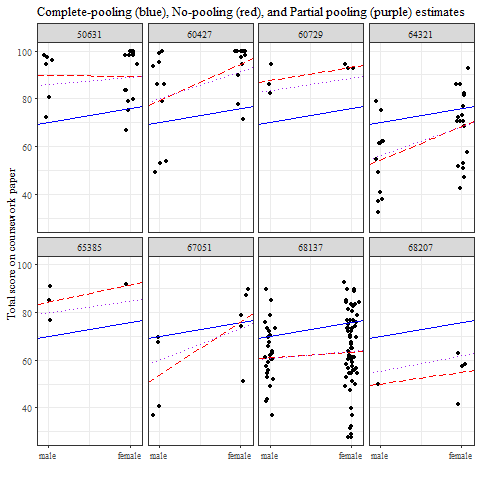
\includegraphics[width=10cm,height=10cm,keepaspectratio]{graphics/pooling.png}
	\caption{We see that the estimated school-specific regression line from the partial pooling estimates lies between the complete-pooling and no-pooling regression lines. There is more pooling (purple dotted line closer to red dotted line) in schools with larger sample sizes.}
	\label{fig:pooling}
\end{figure}

\begin{figure}
	\centering
	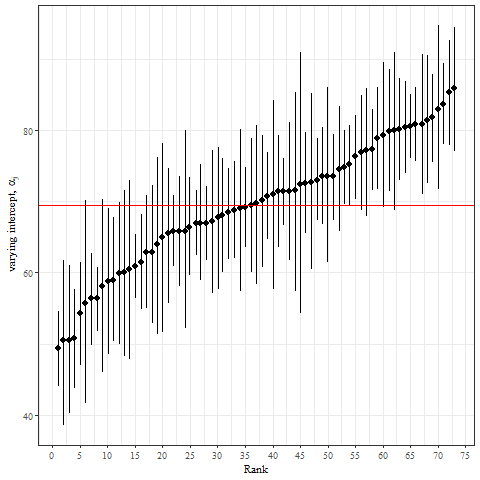
\includegraphics[width=10cm,height=10cm,keepaspectratio]{./graphics/ranking.png}
	%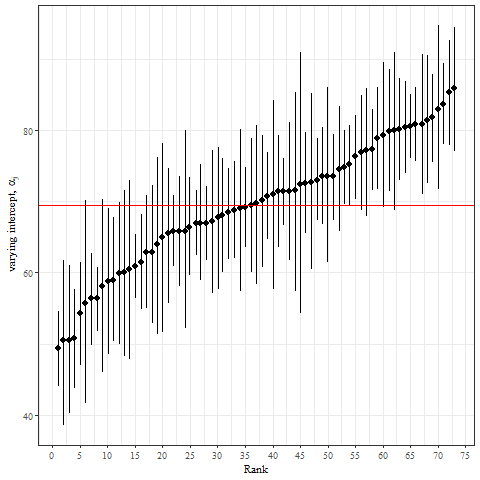
\includegraphics[width=\linewidth]{graphics/ranking.png}
	\caption{Ranking for school varying intercepts. The red line represents the mean of all the posterior means: $69.42577$.}
	\label{fig:ranking}
\end{figure}

\begin{figure}
	\centering
	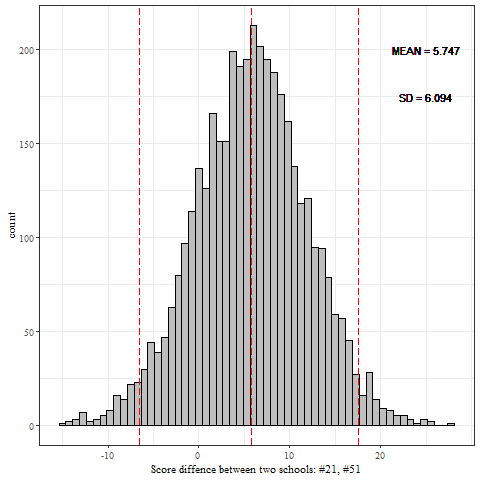
\includegraphics[width=10cm,height=10cm,keepaspectratio]{graphics/differences.png}
	\caption{}
	\label{fig:differences}
\end{figure}

\begin{figure}
	\centering
	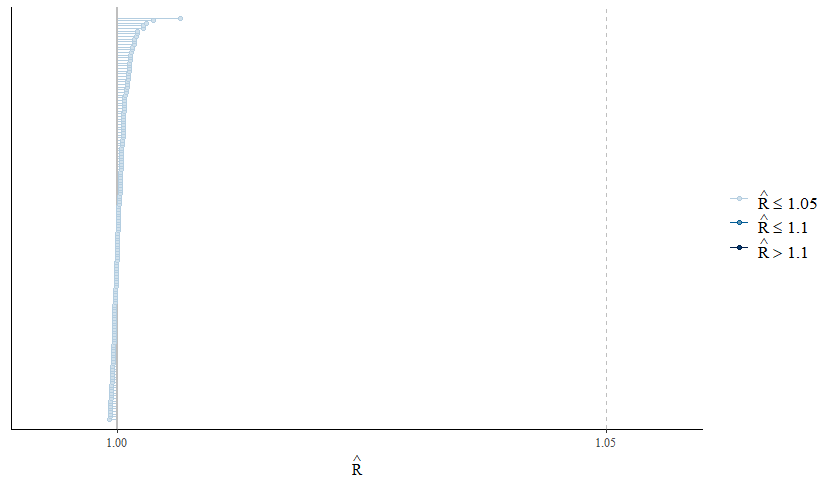
\includegraphics[width=15cm,height=15cm,keepaspectratio]{graphics/rhat.png}
	\caption{The ratio of between-chain variance to within-chain variance.}
	\label{fig:rhat}
\end{figure}
=======
%\begin{figure}[ht]
%\begin{center}
%\begin{tikzpicture}%
%  [vertex/.style={circle,draw=black,fill=white, minimum size=1cm},
%  node distance=2.5cm,
%  >=latex,
%  on grid]
%  \node[vertex] (phi) {$\mu, \tau^2$};
%  \node[vertex,below left=1.5cm and 2cm of phi] (theta1) {$\theta_1$};
%  \node[vertex,below right=1.5cm and 2cm of phi] (thetaJ) {$\theta_J$};
%  \node[below=1.5cm of phi] (dots1) {$\dots$};
%  \node[vertex,below=2cm of theta1] (y1) {$y(1)$};
%  \node[vertex,below=2cm of thetaJ] (yJ) {$y(J)$};
%  \node[rectangle, draw=black, minimum size=0.8cm, below=2.5cm of phi] (sigma) {$\sigma^2$};
%  \node[below=3.5cm of phi] (dots1) {$\dots$};
%  \draw[->]
%    (phi) edge (theta1)
%    (phi) edge (thetaJ)
%    (theta1) edge (y1)
%    (thetaJ) edge (yJ)
%    (sigma) edge (y1)
%    (sigma) edge (yJ);
%\end{tikzpicture}
%\end{center}
%\label{fig:example_model}
%\caption{The directed acyclical graph representation of the model structure of the example model in subsection \ref{sec:hierachical_solving}. Random  and fixed quantities are depicted in circles and squares, respectively.}
%\end{figure}
>>>>>>> ebcc425e29d80a0c61f20838e55b994abb056eb1

\subsection{Tables}

\begin{proof}[Derivation of Results in Table \ref{tab:comp_uniform_bay_ml}.]
  For the normal distributed data problem at hand the derivation of the maximum likelihood estimators, $\bar{y}$ for $\mu$ and $(n-1) s^2 / n$ for $\sigma^2$, is well known.
  We note that the "ML Variance" denotes the theoretical variance of the estimators.
  Further, the moments of the scaled inverse $\chi^2$ distributions are available in closed form.
  In particular, if $X \sim \scaledInvChi{\nu, \tau^2}$, then $\Exp{X} = \nu \tau^2 / (\nu - 2)$ and $\var{X} = 2 \nu^2 \tau^4 / ((\nu - 2)^2 (\nu - 4))$.

  Let us first consider the parameter $\mu$.
  As the t-distribution is parameterized over its mean and variance we can simply read off these values.
  Further, as the t-distribution is symmetric the MAP is equal to its mean.

  Let us now consider the parameter $\sigma^2$.
  Plugging in the respective parameters, we get
  \begin{align*}
    \Exp{\sigma^2 \mid y} = \frac{n - 1}{n - 3} \sigma^2
  \end{align*}
  directly, and
  \begin{align*}
    \var{\sigma^2 \mid y} = \frac{2 (n-1)^2}{(n-3)^2(n-5)} \sigma^4 \,.
  \end{align*}
  To get the MAP for $\sigma^2$ we need to maximize the posterior of $\sigma^2$.
  Note that we can drop any integration constants, i.e. we need to solve
  \begin{align*}
    \maximize_{x > 0} \left\{x^{-(1 + \frac{n-1}{2})} \EXP{\frac{-(n-1) s^2}{2 x}}\right\} \,,
  \end{align*}
  where the term in curly brackets is just the posterior density of $\sigma^2$ evaluated at $x$.
  Differentiating with respect to $x$ and setting this to zero yields the desired result.
\end{proof}

\begin{proof}[Derivation of Results in Table \ref{tab:comp_conjugate_bay_ml}.]
  The proof from above applies here by mutatis mutandis.
\end{proof}

%\begin{proof}[Derivation of Results in Table \ref{tab:vol_high_dim}]
%See file \lstinline{volume.py}{} in the online appendix.
%\end{proof}

\subsection{Proofs}
\begin{remark}
The proofs presented here follow \citet{gelmanbda04}; however, we contribute detailed remarks.
\end{remark}

\begin{proof}[Proof of Proposition \ref{prop:posterior_uniform}.]
  Consider first the object $\mu \mid \sigma^2, y$.
  We get
  \begin{align*}
    p(\mu \mid \sigma^2, y) \propto p(y \mid \mu, \sigma^2) p(\mu \mid \sigma^2) \propto p(y \mid \mu, \sigma^2) \,,
  \end{align*}
  where the last step follows as the priors are assumed to be independent.
  Note then
  \begin{align*}
    p(\mu \mid \sigma^2, y) &\propto \EXP{-\frac{1}{\sigma^2}\sum_i (y_i - \mu)^2} = \EXP{-\frac{n}{\sigma^2} \frac{1}{n}\sum_i (y_i^2 - 2y_i \mu + \mu^2)}\\
    &=\EXP{-\frac{n}{\sigma^2} (\bar{y^2} - 2 \bar{y} \mu + \mu^2)} \propto
    \EXP{-\frac{1}{\sigma^2 / n} (\mu - \bar{y})^2} \,,
  \end{align*}
  where $\bar{y^2} = \frac{1}{n}\sum_i y_i^2$ and the last step is only proportional as we switch $\bar{y^2}$ for $\bar{y}^2$.
  Note that proportionality here is with respect to $\mu$.
  We thus get $\mu \mid \sigma^2, y \sim \normal{\bar{y}, \sigma^2/n}$ as our first intermediate result.

  Consider now $\sigma \mid y$.
  As we already derived the joint posterior we can compute the marginal posterior of $\sigma^2$ by integrating out $\mu$.
  Note that $\sum_i (y_i - \mu)^2 = [(n-1)s^2 + n(\bar{y} - \mu)^2]$, where $s^2$ denotes the (unbiased) sample variance. Hence
  \begin{align*}
    p(\sigma^2 \mid y) &\propto \int p(\mu, \sigma^2 \mid y) \mathrm{d} \mu\\
    &\propto \int \sigma^{-(n+2)} \EXP{-\frac{1}{2\sigma^2}\sum_i (y_i - \mu)^2} \mathrm{d} \mu\\
    &= \sigma^{-(n+2)} \int \EXP{-\frac{1}{2\sigma^2}\sum_i (y_i - \mu)^2} \mathrm{d} \mu\\
    &= \sigma^{-(n+2)} \int \EXP{-\frac{1}{2\sigma^2}[(n-1) s^2 + n(\bar{y} - \mu)^2]} \mathrm{d} \mu\\
    &= \sigma^{-(n+2)} \EXP{-\frac{1}{2\sigma^2}[(n-1) s^2]} \int \EXP{\frac{1}{2\sigma^2/n}(\mu - \bar{y})^2} \mathrm{d} \mu\\
    &= \sigma^{-(n+2)} \EXP{-\frac{1}{2\sigma^2}[(n-1) s^2]} \sqrt{2 \pi \sigma^2 / n} \\
    &\propto (\sigma^2)^{-(n+1)/2} \EXP{-\frac{1}{2\sigma^2}[(n-1) s^2]} \,,
  \end{align*}
  where the second to last step follows simply by considering the constant of integration of the normal distribution of $\mu \mid \sigma^2, y$.
  Note that here we consider proportionality with respect to $\sigma^2$.
  By inspection we see that $\sigma^2 \mid y \sim \text{scaled-Inv-} \chi^2(n-1, s^2)$, which proves our first claim.

  To finish the proof we integrate the joint posterior over $\sigma^2$ to get the marginal posterior of $\mu$.
  We evaluate the integral by substitution using
  $z = \sfrac{a}{2 \sigma^2}$ with $a = (n-1)s^2 + n(\mu - \bar{y})^2$.

  Then,
  \begin{align*}
    p(\mu \mid y) &= \int_{(0, \infty)} p(\mu, \sigma^2 \mid y) \mathrm{d}\sigma^2\\
    &\propto  \int_{(0, \infty)} (\sigma^2)^{-(n+2)/2} \EXP{-\frac{1}{2\sigma^2}[(n-1) s^2 + n(\mu - \bar{y})^2]} \mathrm{d} \sigma^2\\
    &\propto \int_{(0, \infty)} (\sigma^2)^{-(n+2)/2}\EXP{-z} [(\sigma^2)^2 / a] \mathrm{d}z\\
    &= \int_{(0, \infty)} (\sigma^2)^{-(n-2)/2} / a \EXP{-z} \mathrm{d}z\\
    &= a^{-n/2}\int_{(0, \infty)} z^{(n-2)/2}\EXP{-z} \mathrm{d}z\\
    &= a^{-n/2} \, \Gamma(n/2)\\
    &\propto a^{-n/2}\\
    &= [(n-1)s^2 + n(\mu - \bar{y})^2]^{-n/2}\\
    &\propto \left[1 + \frac{1}{n-1} \frac{(\mu - \bar{y})^2}{s^2 / n}\right]^{-n/2} \,
  \end{align*}
  where $\Gamma$ denotes the gamma function (which is finite on the positive real numbers).
  This concludes the proof by implying that $\mu \mid y \sim t_{n-1}(\bar{y}, s^2/n)$,
\end{proof}


\begin{proof}[Proof of Proposition \ref{prop:posterior_conjugate}.]
Let us first state equation \ref{eq:conjugate_posterior} and the premise again.
We have to show that
\begin{align*}
  p(\mu, \sigma^2 \mid y) \propto& (\sigma^2)^{-\frac{3 + \nu_0 + n}{2}} \times\\
  & \times \EXP{-\frac{1}{2 \sigma^2} \left[\nu_0\sigma_0^2 + \kappa_0(\mu - \mu_0)^2 + (n-1)s^2 + n(\bar{y} - \mu)^2 \right]}
\end{align*}
is $\NormalscaledInvChi{\mu_n, \sigma_n^2/\kappa_n; \nu_n, \sigma_n^2}$ with $\nu_n = \nu_0 + n$, $\kappa_n = \kappa_0 + n$, $\mu_n =\frac{\kappa_0}{\kappa_0 + n}\mu_0 + \frac{n}{\kappa_0 + n}\bar{y}$, $\sigma_n^2 = \left[\nu_0 \sigma_0^2 + (n-1)s^2 + \frac{\kappa_0 n}{\kappa_0 + n} (\bar{y} - \mu_0)^2\right] /\nu_n$.
By definition of the normal-scaled-inverse-$\chi^2$ distribution $\nu_n = \nu_0 + n$ follows trivially.
Let us therefore consider the term in square brackets in the exponential.
We have to show that
\begin{align*}
  \left[\nu_0\sigma_0^2 + \kappa_0(\mu - \mu_0)^2 + (n-1)s^2 + n(\bar{y} - \mu)^2 \right] = \nu_n \sigma_n^2 + \kappa_n (\mu - \mu_n)^2 \,.
\end{align*}
Plugging in for $\sigma_n^2$ we get for the right-hand side
\begin{align*}
  \nu_n \sigma_n^2 + \kappa_n (\mu - \mu_n)^2 = \nu_0 \sigma_0^2 + (n-1)s^2 + \frac{\kappa_0 n}{\kappa_0 + n} (\bar{y} - \mu_0)^2 + \kappa_n (\mu- \mu_n)^2 \,.
\end{align*}
Therefore we only need to check
\begin{align*}
  \kappa_0(\mu - \mu_0)^2 + n(\bar{y} - \mu)^2 = \frac{\kappa_0 n}{\kappa_0 + n} (\bar{y} - \mu_0)^2 + \kappa_n (\mu- \mu_n)^2 \,.
\end{align*}
Expanding the right-hand side we get
\begin{align*}
\frac{\kappa_0 n}{\kappa_0 + n} &(\bar{y} - \mu_0)^2 + \kappa_n (\mu- \mu_n)^2\\
&=\frac{\kappa_0 n}{\kappa_n}\left[\bar{y}^2 - 2\bar{y}\mu_0 + \mu_0^2 \right] + \kappa_n \left[\mu^2 - 2\mu\mu_n + \mu_n^2 \right]\\
&=\frac{\kappa_0 n}{\kappa_n}\left[\bar{y}^2 - 2\bar{y}\mu_0 + \mu_0^2 \right] + \kappa_n \left[\mu^2 - 2\mu\frac{\kappa_0}{\kappa_n}\mu_0 - 2\mu\frac{n}{\kappa_n}\bar{y} + \frac{\kappa_0^2}{\kappa_n^2}\mu_0^2 + \frac{n^2}{\kappa_n^2} \bar{y}^2 + 2\frac{\kappa_0}{\kappa_n} \frac{n}{\kappa_n}\mu_0\bar{y} \right]\\
&=\frac{\kappa_0 n}{\kappa_n}\left[\bar{y}^2 - 2\bar{y}\mu_0 + \mu_0^2 \right] + \kappa_n \mu^2 - 2\mu \kappa_0 \mu_0 - 2\mu n\bar{y} + \frac{\kappa_0^2}{\kappa_n}\mu_0^2 + \frac{n^2}{\kappa_n} \bar{y}^2 + 2 \kappa_0 n \mu_0 \bar{y} / \kappa_n\\
&= \left(\kappa_0 \mu^2 -2\mu \kappa_0 \mu_0 \right) + \left(n \mu^2 - 2 n \mu \bar{y} \right) + \frac{\kappa_0 n}{\kappa_n}\bar{y}^2 + \frac{\kappa_0 n}{\kappa_n}\mu_0^2 + \frac{\kappa_0^2}{\kappa_n} \mu_0^2 + \frac{n^2}{\kappa_n} \bar{y}^2\\
&= \left(\kappa_0 \mu^2 -2\mu \kappa_0 \mu_0 \right) + \left(n \mu^2 - 2 n \mu \bar{y} \right) + \bar{y}^2 \left(\frac{\kappa_0 n}{\kappa_n} + \frac{n^2}{\kappa_n}\right) + \mu_0^2\left(\frac{\kappa_0 n}{\kappa_n} + \frac{\kappa_0^2}{\kappa_n}\right)\\
&= \left(\kappa_0 \mu^2 -2\mu \kappa_0 \mu_0 + \kappa_0 \mu_0^2 \right) + \left(n \mu^2 - 2 n \mu \bar{y} + n \bar{y}^2\right)\\
&=\kappa_0(\mu - \mu_0)^2 + n(\bar{y} - \mu)^2 \,,
\end{align*}
which was what we wanted.
\end{proof}

\begin{proof}[Proof of Proposition \ref{prop:marginal_posterior}.]
We continue to use the notation of the previous proof.
As in the proof of proposition \ref{prop:posterior_uniform} we first compute the distribution of $\mu \mid \sigma^2, y$ and then derive the posterior of $\sigma^2$ by integrating $\mu$ out.
Note that we actually defined $\mu \mid \sigma^2 \sim \normal{\mu_0, \sigma^2/\kappa_0}$.
Hence,
\begin{align*}
  p(\mu \mid \sigma^2, y) &\propto p(y \mid \mu, \sigma^2) p(\mu \mid \sigma^2)\\
  &\propto \EXP{-\frac{1}{2\sigma^2/n} (\mu - \bar{y})^2} \EXP{-\frac{1}{2\sigma^2/\kappa_0}(\mu - \mu_0)^2}\\
  &= \EXP{-\frac{1}{2\sigma^2}\left[n(\mu - \bar{y})^2 + \kappa_0(\mu - \mu_0)^2 \right]}\\
  &= \EXP{-\frac{1}{2\sigma^2}\left[\mu^2(\kappa_0 + n) - 2\mu(\kappa_0\mu_0 + n\bar{y}) + (\mydots) \right]}\\
  &= \EXP{-\frac{1}{2\sigma^2 / \kappa_n}\left[\mu^2 - 2\mu(\kappa_0\mu_0 + n\bar{y})/\kappa_n + (\mydots)/\kappa_n \right]}\\
  &= \EXP{-\frac{1}{2\sigma^2 / \kappa_n}\left(\mu - \mu_n^2\right) + (\mydots)}\\
  &\propto \EXP{-\frac{1}{2\sigma^2 / \kappa_n}\left(\mu - \mu_n^2\right)} \,,
\end{align*}
which implies that $\mu \mid \sigma^2, y \sim \normal{\mu_n, \sigma^2 / \kappa_n}$, where we used $(\mydots)$ to denote constants independent of $\mu$.

Now we can use this result as
\begin{align*}
  p(\sigma^2 \mid y) &= \int p(y, \sigma^2 \mid y) \mathrm{d}\mu\\
  &\propto \int (\sigma^2)^{-\frac{3 + \nu_n}{2}} \EXP{\frac{1}{2\sigma^2} \left[\nu_n \sigma_n^2 + \kappa_n(\mu_n - \mu)^2 \right]}\mathrm{d}\mu\\
  &\propto (\sigma^2)^{-\frac{3 + \nu_n}{2}} \int \EXP{\frac{1}{2\sigma^2} \nu_n \sigma_n^2}\EXP{\frac{1}{2\sigma^2 / \kappa_n} (\mu_n - \mu)^2 }\mathrm{d}\mu\\
  &\propto (\sigma^2)^{-\frac{3 + \nu_n}{2}}\EXP{\frac{1}{2\sigma^2} \nu_n \sigma_n^2} \int \EXP{\frac{1}{2\sigma^2 / \kappa_n} (\mu_n - \mu)^2 }\mathrm{d}\mu\\
  &\propto (\sigma^2)^{-\frac{3 + \nu_n}{2}}\EXP{\frac{1}{2\sigma^2} \nu_n \sigma_n^2} \sqrt{2 \pi \sigma^2 / \kappa_n}\\
  &\propto (\sigma^2)^{-(1 + \frac{\nu_n}{2})} \EXP{-\frac{1}{2\sigma^2}\nu_n\sigma_n^2}\,,
\end{align*}
from which we can conclude that $\sigma^2 \mid y \sim \scaledInvChi{\nu_n, \sigma_n^2}$.

We end the proof by deriving the marginal posterior of $\mu$ using an analogous approach as in the proof of Proposition \ref{prop:posterior_uniform}.
Define $a := \left[\nu_n\sigma_n^2 + \kappa_n(\mu_n - \mu)^2 \right]$. We solve for the posterior by integrating $\sigma^2$ out using the substitution $z = \frac{a}{2\sigma^2}$. Then
\begin{align*}
  p(\mu \mid y) &= \int_{(0, \infty)} p(\mu, \sigma^2 \mid y) \mathrm{d}\sigma^2\\
  &\propto \int_{(0, \infty)}(\sigma^2)^{-\frac{3 + \nu_n}{2}} \EXP{\frac{1}{2\sigma^2} \left[\nu_n \sigma_n^2 + \kappa_n(\mu_n - \mu)^2 \right]}\mathrm{d}\sigma^2\\
  &\propto \int_{(0, \infty)}(\sigma^2)^{-\frac{3 + \nu_n}{2}} \EXP{\frac{a}{2\sigma^2}}\mathrm{d}\sigma^2\\
  &\propto \int_{(0, \infty)}(a / 2z)^{-\frac{3 + \nu_n}{2}} \EXP{-z} \frac{a}{2 z^2} \mathrm{d}z\\
  &\propto \int_{(0, \infty)}a^{-\frac{3 + \nu_n}{2}}a z^{\frac{3 + \nu_n}{2}}z^{-2} \EXP{-z} \mathrm{d}z\\
  &= a^{-\frac{1 + \nu_n}{2}} \int_{(0, \infty)} z^{\frac{\nu_n - 1}{2}} \EXP{-z} \mathrm{d}z\\
  &= a^{-\frac{1 + \nu_n}{2}} \Gamma\left(\frac{\nu_n + 1}{2}\right)\\
  &\propto a^{-\frac{1 + \nu_n}{2}}\\
  &= \left[\nu_n \sigma_n^2 + \kappa_n(\mu_n - \mu)^2 \right]^{-\frac{1 + \nu_n}{2}}\\
  &= \left[\nu_n \sigma_n^2\left(1 + \frac{1}{\nu_n}\frac{(\mu_n - \mu)^2}{\sigma_n^2 / \kappa_n}\right) \right]^{-\frac{1 + \nu_n}{2}}\\
  &\propto \left[1 + \frac{1}{\nu_n}\frac{(\mu_n - \mu)^2}{\sigma_n^2 / \kappa_n} \right]^{-\frac{1 + \nu_n}{2}} \,,
\end{align*}
which concludes the proof by implying that $\mu \mid y \sim t_{\nu_n}(\mu_n, \sigma_n^2 / \kappa_n)$.
\end{proof}

%\begin{proof}[Proof of Proposition \ref{prop:hierarchical_posterior}.]
%  Let us first consider the parameter definitions again for clarity.
%  We define
%  \begin{align*}
%    \sigma_\mu^{-2} = \sum_j \frac{1}{\sigma_j^2 + \tau^2}\,,\,\, \tau_j^{-2}=\frac{1}{\sigma_j^2} + \frac{1}{\tau^2}\,,\,\, \mu_j=\tau_j^2(\frac{1}{\sigma_j^2} \bar{y}_j + \frac{1}{\tau^2}\mu) \,,\,\, \bar{\mu} = \sigma_\mu^2 \sum_j \frac{1}{\sigma_j^2 + \tau^2} \bar{y}_j \,.
%  \end{align*}
%  \noindent
%  \textbf{\emph{i.)}} Note that $p(\theta \mid \mu, \tau^2, y) \propto p(y \mid \theta, \mu, \tau^2) p(\theta \mid \mu, \tau^2) = p(y \mid \theta) p(\theta \mid \mu, \tau^2)$, as conditional on $\theta$ the observations and hyperparameter are independent.
%  Now by construction we get $p(\theta \mid \mu, \tau^2) = \prod_j p(\theta_j \mid \mu, \tau^2)$.
%  Note that since we assume independence we clearly also get $p(\theta \mid \mu, \tau^2, y) = \prod_j p(\theta_j \mid \mu, \tau^2, y)$; however to get the distribution of $p(\theta_j \mid \mu, \tau^2, y)$ we split the likelihood into factors dependent only on $\theta_j$ and show that the product of the factors constitutes a normal density with the desired parameters.
%  So we have to show that $p(y \mid \theta)$, considered as a function of $\theta$, factors into $J$ factors each only dependent on $\theta_j$.
%  Denoting terms not dependent on the $\theta_j's$ by $(\mydots)$, we get
%  \begin{align*}
%    p(y \mid \theta) &= \prod_{i=1}^n p(y_i \mid \theta)=\prod_{i=1}^n p(y_i \mid \theta_{j[i]}) = \prod_{j=1}^J \prod_{i:j[i]=j} p(y_i \mid \theta_{j})\\
%    &= \prod_j (2 \pi \sigma^2)^{-n_j / 2} \EXP{-\frac{1}{2\sigma^2}\sum_{i:j[i]=j} (y_i - \theta_j)^2}\\
%    &\propto \prod_j \EXP{-\frac{1}{2\sigma^2} \left[n_j \theta_j^2 - n_j 2\theta_j\bar{y}_j + (\mydots)\right]}\\
%    &\propto \prod_j \EXP{-\frac{1}{2\sigma^2 / n_j} (\theta_j - \bar{y}_j)^2} \,.
%  \end{align*}
%  Hence,
%  \begin{align*}
%    p(\theta \mid \mu, \tau^2, y) &\propto p(y \mid \theta) p(\theta \mid \mu, \tau^2)\\
%    &\propto \prod_j \EXP{-\frac{1}{2\sigma^2 / n_j} (\theta_j - \bar{y}_j)^2} \prod_j p(\theta_j \mid \mu, \tau^2)\\
%    &\propto \prod_j \EXP{-\frac{1}{2\sigma^2 / n_j} (\theta_j - \bar{y}_j)^2} \EXP{-\frac{1}{2\tau^2}(\theta_j - \mu)^2}\\
%    &= \prod_j \EXP{-\frac{1}{2\sigma^2 / n_j} (\theta_j - \bar{y}_j)^2 -\frac{1}{2\tau^2}(\theta_j - \mu)^2}\\
%    &= \prod_j \EXP{-\frac{1}{2}\left[\left(\frac{1}{\sigma^2/n_j} + \frac{1}{\tau^2}\right)\theta_j^2 - 2\theta_j\left(\frac{1}{\sigma^2/n_j}\bar{y}_j + \frac{1}{\tau^2}\mu\right) + (\mydots) \right]}\\
%    &= \prod_j \EXP{-\frac{1}{2}\left[\tau_j^{-2} \theta_j^2 - 2\theta_j\mu_j\tau_j^{-2} + (\mydots) \right]}\\
%    &\propto \prod_j \EXP{-\frac{1}{2\tau_j^2} (\theta_j - \mu_j)^2} \,,
%  \end{align*}
%which gives $\theta_j \mid \mu, \tau^2, y \sim \normal{\mu_j, \tau_j^2}$.\\
%
%  \noindent
%  \textbf{\emph{ii.)}} Let us first prove an intermediate result, namely $\bar{y}_j \mid \mu, \tau^2 \sim \normal{\mu, \sigma_j^2 + \tau^2}$ for all $j$.
%  Note that we may write
%  \begin{align*}
%    p(\bar{y}_j \mid \mu, \tau^2) &= \int p(\bar{y}_j, \theta_j \mid \mu, \tau^2)\mathrm{d}\theta_j = \int p(\bar{y}_j \mid \theta_j) p(\theta_j \mid \mu, \tau^2)\mathrm{d}\theta_j \,.
%  \end{align*}
%  We know that $\bar{y}_j \mid \theta_j \sim \normal{\theta_j, \sigma_j^2}$ and $\theta_j \mid \mu, \tau^2 \sim \normal{\mu, \tau^2}$, which means that we can factor the term in the integral into an exponential containing a quadratic term in $\bar{y}_j$ (and not $\theta_j$) and an expontential containing a quadratic term in $\theta_j$.
%  The former term we may pull out of the intgral and the latter disappears into a constant (not depending on $\bar{y}_j$) as we integrate over $\theta_j$.
%  We omit a detailed derivation here and refer to \citet{gelmanbda04}.
%
%  Then using that for $j=1,\mydots,J$ the quantities $\bar{y}_j \mid \mu, \tau^2$ are independent, we can write
%  \begin{align*}
%    p(\mu, \tau^2 \mid y) \propto p(y \mid \mu, \tau^2) p(\mu, \tau) = \prod_j p(\bar{y}_j \mid \mu, \tau^2) p(\mu \mid \tau) p(\tau) \propto p(\tau) \prod_j p(\bar{y}_j \mid \mu, \tau^2) \,,
%  \end{align*}
%  where we use that $p(\mu \mid \tau) \propto 1$.
%  Note that we can also write $p(\mu, \tau \mid y) = p(\mu \mid \tau, y) p(\tau \mid y)$.
%  Therefore we get
%  \begin{align*}
%    p(\mu \mid \tau, y) p(\tau \mid y) \propto p(\tau) \prod_j p(\bar{y}_j \mid \mu, \tau^2) \,.
%  \end{align*}
%  Now if we consider the factors depending on $\mu$ more closely we see that (using equivalent transformations as above and plugging in the definitions)
%  \begin{align*}
%    \prod_j p(\bar{y}_j \mid \mu, \tau^2) &\propto \prod_j \EXP{-\frac{1}{2(\sigma_j^2 + \tau^2)}(\bar{y}_j - \mu)^2}\\
%    &=\EXP{-\frac{1}{2}\sum_j \frac{1}{\sigma_j^2 + \tau^2}(\bar{y}_j - \mu)^2}\\
%    &\propto \EXP{-\frac{1}{2 \sigma_\mu^2} (\mu - \bar{\mu})^2}
%  \end{align*}
%  where proportionality is with respect to $\mu$.
%  As we can factor $p(\mu \mid \tau^2, y)$ and as $\mu$ only appears as a quadratic in the exponential we may derive that $\mu \mid \tau^2, y \sim \normal{\bar{\mu}, \sigma_\mu^2}$, which was what we wanted.
%
%  \noindent
%  \textbf{\emph{iii.)}}
%
%\end{proof}
